\input{preambule-sacha-utf8.ltx}

\usepackage{parcolumns}

        \title {Démonstrations de terminale S - Tronc commun \\
                Lycée International}

        \author{Sacha Dhénin}
        
\usepackage{amsthm}
\usepackage{tikzsymbols}

\begin{document}

%\iffalse

\pgfmathdeclarefunction{gauss}{2}{%
  \pgfmathparse{1/(#2*sqrt(2*pi))*exp(-((\x-#1)^2)/(2*#2^2))}%
}

%\maketitle
\newpage
%\thispagestyle{empty}

%\fi

% POUR LES FIGURES : 
%\def\myscale{.75} % par défaut 
%\newcommand{\myfigure}[2]{  % entrée : echelle, fichier figure
%\def\myscale{#1}\begin{center}\footnotesize{#2}\end{center}}
%\newcommand{\E}{(-4,-1) rectangle (4,4)}
%\newcommand{\A}{(0,0) ++(135:2) circle (1.9)}
%\newcommand{\B}{(0,0) ++(45:2) circle (1.9)}
%\definecolor{myred}{rgb}{0,0,0}
%\definecolor{myorange}{rgb}{0,0,0}

\thispagestyle{empty}

%\setcounter{tocdepth}{4}
%\tableofcontents

%\newpage 

%Remplacer tous les $\varnothing$ par $\emptyset$.

\newpage

\vspace*{-2cm}

\section*{Étude graphique des trinômes du seconde degré}


\subsection*{Premier cas}

Soit $f$ la fonction définie par $f(x) = ax^2 + bx + c$. 

\bigskip 

\begin{tikzpicture}[line cap=round,line join=round,>=triangle 45,x=1.0cm,y=1.0cm]
\draw [color=gray!75,dash pattern=on 2pt off 2pt, xstep=1.0cm,ystep=1.0cm] (-7,-5.5) grid (10,8.5);
\draw[->] (-7,0.) -- (10,0.);
\foreach \x in {-6,...,-1,1,2,...,10}
\draw[shift={(\x,0)}] (0pt,2pt) -- (0pt,-2pt) node[below] {\footnotesize $\x$};
\draw[->] (0.,-5.5) -- (0.,8.5);
\foreach \y in {-5,-4,-3,-2,-1,1,2,3,4,5,6,7,8}
\draw[shift={(0,\y)}] (2pt,0pt) -- (-2pt,0pt) node[left] {\footnotesize $\y$};
\draw(0pt,-10pt) node[right] {\footnotesize $0$};
\clip(-7,-4.5) rectangle (10,8.58);
% f(x) > 5 
 \draw [ultra thick, samples=50,rotate around={0.:(1.,-4.)},xshift=1.cm,yshift=-4.cm,color=Orchid,domain=-3.6:-3.0)] plot (\x,{(\x)^2/2/0.5});
  \draw [ultra thick, samples=50,rotate around={0.:(1.,-4.)},xshift=1.cm,yshift=-4.cm,color=Orchid,domain=3.0:3.6)] plot (\x,{(\x)^2/2/0.5});
% 0 < f(x) < 5   
  \draw [samples=50,rotate around={0.:(1.,-4.)},xshift=1.cm,yshift=-4.cm,color=red,domain=-3.0:-2)] plot (\x,{(\x)^2/2/0.5});
  \draw [samples=50,rotate around={0.:(1.,-4.)},xshift=1.cm,yshift=-4.cm,color=red,domain=2.0:3)] plot (\x,{(\x)^2/2/0.5});
% f(x) < 0 
 \draw [ultra thick, samples=50,rotate around={0.:(1.,-4.)},xshift=1.cm,yshift=-4.cm,color=DarkOrange,domain=-2:2)] plot (\x,{(\x)^2/2/0.5});  
 % Ensemble de solutions 
 \draw [ultra thick, color=DeepPink](-7,0) -- (-2,0) ;   
 \draw [ultra thick, color=DeepPink](4,0) -- (10,0) ;    
\draw [ultra thick, color=green](-1,0) -- (3,0) ;    
% 
\draw [color=darkgreen,domain=-7:10] plot(\x,{(5.-0.*\x)/1.});
\draw (-5.3,8) node[anchor=north west] {$y = ax^2 + bx + c$};
\draw (7,5) node[anchor=north west] {$y = 5$};
\begin{scriptsize}
\draw  (1.,-4.) circle (1.5pt);
\draw(1,-4.1)[below] node {$S$};
\draw [fill] (-2.,5.) circle (1.5pt);
\draw [fill] (4.,5.) circle (1.5pt);
\end{scriptsize}
 \draw [ thick, dashed, color=DarkBlue](1,0) -- (1,-4) -- (0,-4) ;  
\draw (-1,0) node  {\color{blue} $\times$} ;  \draw (-1,0) node [above right] {\color{blue} $x_1$} ; 
\draw ( 1,0) node  {\color{blue} $\times$} ;  \draw ( 1,0) node [above right] {\color{blue} $\alpha$} ; 
\draw ( 3,0) node  {\color{blue} $\times$} ;  \draw ( 3,0) node [above right] {\color{blue} $x_2$} ; 
\draw (0,-3) node  {\color{blue} $\times$} ;  \draw (0,-3) node [above right] {\color{blue} $c$} ; 
\draw (0,-4) node  {\color{blue} $\times$} ;  \draw (0,-4) node [below left] {\color{blue} $\beta$} ; 
\end{tikzpicture}

\medskip 

\setbox1=\vbox{\hsize=15mm\begin{center} \dChangey[3]{2}\\ {\it Think positive}\end{center}}

\setbox2=\hbox{$\left\lbrace \begin{array}{lr}
x_1 = & -1 \\
x_2 = & 3
\end{array} \right.$}
\begin{enumerate}
\item Que vaut $a$ ? Ici, $a$ est négatif  : $\vcenter{\box1}$
\item Que vaut $c$ ? $f(0)=3$ donc,i $c=3$. 
\item Que vaut $\alpha$ ? $\alpha$ est l'abscisse du sommet $\longrightarrow$ ici $\alpha=1$. 
\item Que vaut $\beta$ ? $\beta$  est l'ordonnée du sommet  $\beta=f(\alpha) \longrightarrow$ ici $\beta=-4$. 
\item Quelles sont les racines ? Ce sont les abscisses des points d'intersection de la courbe \\avec l'axe des abscisses   $\longrightarrow$ ici $\vcenter{\box2}$. 
\setlength{\fboxrule}{2pt} 
\item Quelles sont les solutions de  \fcolorbox{Orange}{white}{$f(x)\leqslant 0 $} ?   \fcolorbox{green}{white}{$\mathcal{S}=[-1;3] $} 
\item Quelles sont les solutions de  \fcolorbox{Orchid}{white}{$f(x) > 5 $} ?  
 \fcolorbox{DeepPink}{white}{$\mathcal{S}=]-\infty; -1[ \cup ]3; +\infty $} 
\end{enumerate}
\newpage


\subsection*{Deuxième cas}

Soit $f$ la fonction définie par $f(x) = ax^2 + bx + c$. \\


\bigskip 

\begin{tikzpicture}[line cap=round,line join=round,>=triangle 45,x=1.0cm,y=1.0cm]
\draw [color=gray!75,dash pattern=on 2pt off 2pt, xstep=1.0cm,ystep=1.0cm] (-7,-7.5) grid (10,5);
\draw[->] (-7,0.) -- (10,0.);
\foreach \x in {-6,...,-1,1,2,...,10}
\draw[shift={(\x,0)}] (0pt,2pt) -- (0pt,-2pt) node[below] {\footnotesize $\x$};
\draw[->] (0.,-7.5) -- (0.,5);
\foreach \y in {-7,...,-1,1,2,3,4}
\draw[shift={(0,\y)}] (2pt,0pt) -- (-2pt,0pt) node[left] {\footnotesize $\y$};
\draw(0pt,-10pt) node[right] {\footnotesize $0$};
% f(x)
\draw (-4,-6) node {$y = ax^2 + bx + c$};
\draw [ultra thick,samples=50,rotate around={-180.:(1.,4.)},xshift=9.4mm,yshift=4.cm,color=Orchid,domain=-3.4:-2)] plot (\x,{(\x)^2/2/0.5});
\draw [ultra thick,samples=50,rotate around={-180.:(1.,4.)},xshift=10.7mm,yshift=4.cm,color=Orchid,domain=2:3.4)] plot (\x,{(\x)^2/2/0.5});
\draw [ultra thick,samples=50,rotate around={-180.:(1.,4.)},xshift=10mm,yshift=4.cm,color=Green,domain=-3:3)] plot (\x,{(\x)^2/2/0.5});
% y = -5
\draw (7,-5.5) node {$y = -5$};
\draw [color=darkgreen,domain=-7:10] plot(\x,{(-5.-0.*\x)/1.});
 % Ensemble de solutions 
\draw [ultra thick, color=DeepPink](-7,0) -- (-1,0) ;    \draw [ultra thick, color=DeepPink](3,0) -- (10,0) ;    
\draw [ultra thick, color=green](-1,0) -- (3,0) ;    
%
 \draw [ thick, dashed, color=DarkBlue](1,0) -- (1,4) -- (0,4) ;  
\draw (-1,0) node  {\color{blue} $\times$} ;  \draw (-1,0) node [above right] {\color{blue} $x_1$} ; 
\draw ( 1,0) node  {\color{blue} $\times$} ;  \draw ( 1,0) node [above right] {\color{blue} $\alpha$} ; 
\draw ( 3,0) node  {\color{blue} $\times$} ;  \draw ( 3,0) node [above right] {\color{blue} $x_2$} ; 
\draw (0,3) node  {\color{blue} $\times$} ;  \draw (0,-3) node [above right] {\color{blue} $c$} ; 
\draw (0,4) node  {\color{blue} $\times$} ;  \draw (0,4) node [above right] {\color{blue} $\beta$} ; 
%
\begin{scriptsize}
% \draw  (1.,4.) circle (1.5pt);
\draw(1,4.1)[above] node {$S$};
% \draw [fill] (-2.,5.) circle (1.5pt);
% \draw [fill] (4.,5.) circle (1.5pt);
\end{scriptsize}
\end{tikzpicture}

\medskip 

\setbox1=\vbox{\hsize=15mm\begin{center} \dChangey[3]{-2}\end{center}}

\setbox2=\hbox{$\left\lbrace \begin{array}{lr}
x_1 = & -1 \\
x_2 = & 3
\end{array} \right.$}

\setbox3=\vbox{\hsize=75mm Le sommet $\mathcal{S}$ a pour coordonnées $(1,4)$,\\donc $\alpha = 1$ et $\beta :4$}

\setbox4=\vbox{\hsize=75mm On a $\left\lbrace \begin{array}{l}
f(-1) = 0 \\
f(3) = 0 
\end{array} \right.$, donc $\left\lbrace \begin{array}{l}
x_1 = -1 \\
x_2 = 3 
\end{array} \right.$}

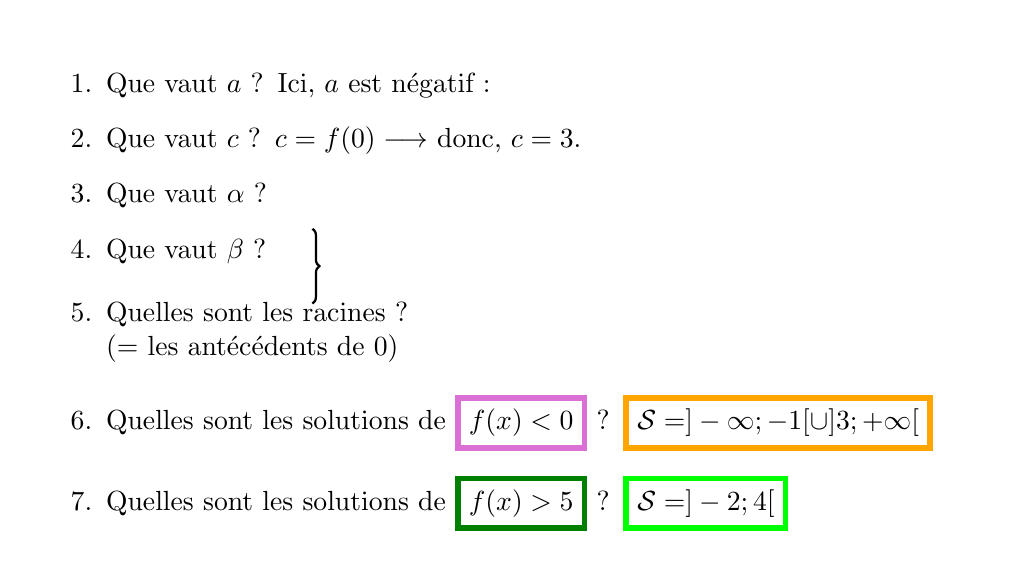
\begin{tikzpicture}[decoration=brace] 
% \draw [color=gray!75,dash pattern=on 2pt off 2pt, xstep=1.0cm,ystep=1.0cm] (0,0) grid (5,5);
 \node[text width=12cm] (box)
{ \begin{enumerate}
\item Que vaut $a$ ? Ici, $a$ est négatif : $\vcenter{\box1}$
\item Que vaut $c$ ? $c=f(0) \longrightarrow$ donc,  $c=3$. 
\item Que vaut $\alpha$ ? 
\item Que vaut $\beta$ ?  \smallskip 
\item Quelles sont les racines ? \\
(= les antécédents de 0) \smallskip 

\setlength{\fboxrule}{2pt} 
\item Quelles sont les solutions de  \fcolorbox{Orchid}{white}{$f(x) <  0 $} ?  
                           \fcolorbox{Orange}{white}{$\mathcal{S}=]-\infty; -1[ \cup ]3; +\infty [ $} 
\item Quelles sont les solutions de  \fcolorbox{Green}{white}{$f(x) > 5 $} ?  
 \fcolorbox{green}{white}{$\mathcal{S}=]-2;4 [$} 
\end{enumerate} } ; % Attention au point-virgule 
% 
\draw [thick, decorate] (-2.5,.7) -- node[right=5pt]{\box3} (-2.5,-.25);
\draw (3.5, -1)  node {\box4} ;
\end{tikzpicture}

\end{document}